\section{Introduction}

Spatial learning is an important function involved in navigation and the formation of episodic memories \cite{spatial_learning_memory}.
The hippocampus and medial entorhinal cortex and implicated for spatial learning due to the presence of the cells that are key for encoding space. Namely cells such as the place cells (for coding locations), grid cells (for distance in a particular direction), head direction cells (heading direction) and boundary cells (for the boundaries of an environment).

\paragraph{Clinical Relevance}

There is evidence that in the early stages of Alzheimer's Disease (AD), visuo-spatial memory impairment is present \cite{Diagnosis}, is partly due to the degeneration of hippocampal cholinergic synaptic transmission \cite{Impairments}.

% and is important in the differential diagnosis of AD.

With greater insight into spatial memory encoding in the brain, it could be possible to come up with a greater understanding of how learning and memory formation occurs more broadly as well as developing improved early clinical diagnosis of AD.

\paragraph{Previous Maze Designs}

Historically, there has been use of the Morris water-maze \cite{morris_water_maze} where a rodent is placed in the water and must navigate to find the platform just beneath the water and navigate towards it, when placed in the water at different points.
The radial arm maze \cite{radial_arm_maze} is an improvement on the T shaped maze \cite{t-maze} which only has to options for choices for the animal to reach, whereas the radial maze is an improvement the animal would have a choice of 7 different places to go when making a decision based on its own cognitive map.

An important improvement that the hexagonal maze is able to bring, is the ability to introduce many more choices for where the animal would like to move to: each time mouse is presented with a decision it can choose between one of two possible choices, however the number of choices of platforms the animal is presented with are unlimited.

% \begin{figure}[h]
%     \centering
%     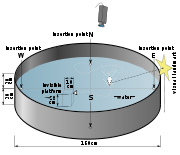
\includegraphics[scale = 0.7]{images/morris_water_maze.png}
%     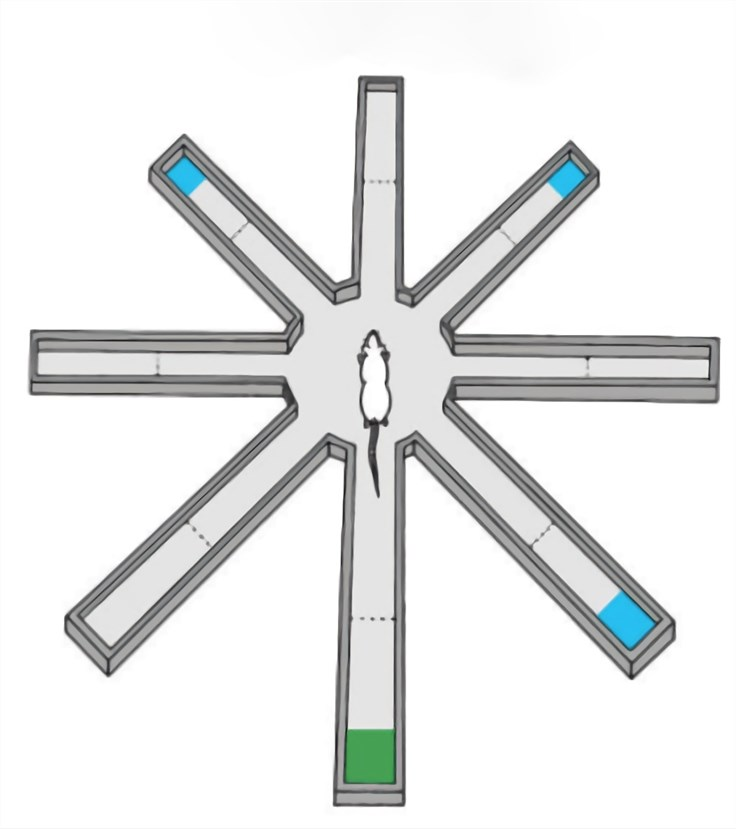
\includegraphics[scale = 0.25]{images/radial_arm_maze.jpg}
%     \caption{Selection of Mazes that have previously been used to investigate how mice encode space in the brain}
%     \label{fig:previousmazes}
% \end{figure}


The hexagonal maze's makes is the ability to respond to the chaning position of the animal poses a great advantage over static mazes such as the radial arm maze where the choices presented to the animal model can not change.
The Honeycomb Maze has been shown to be effective in investigating the cognitive maps of animal models \cite{nature_honeycomb_maze_paper}.

The advantage of the Honeycomb Maze comes at the practical cost of building this maze. This includes the financial cost of making the maze (approx. £100,000) in the laboratory as well as space required to do so.

The proposed solution to this is to use platform robots that are able to dynamically move around each-other. This reduces the cost of building the maze to around £8,000. Further to this, the number of positions the animal model can navigate to is only limited by the size of the room not expensive cost of building more platforms from the previous design.



